\documentclass{article}
\usepackage[utf8]{inputenc}
\usepackage[margin=0.5in]{geometry}
\usepackage{tikz}
\usepackage{amsmath}

\begin{document}
\noindent
Dustin Newman

\noindent
CS 181, Discussion 1C

\noindent
Campbell, Mathur

{\centering
\Large{\textsc{Assignment Six}}
\par}

\section{}
The language described by this PDA is:

$$
L := \{1^20^m10^n \,|\, m = 2n\}
$$

\noindent
Basically, any string which begins with exactly two ones, has some even number of zeroes $m$, exactly one one, and then exactly half of $m$ number of zeroes again, is in the language. Note the interesting parallel where there is twice the number of characters in the $1^20^m$ substring as there is in the $1^10^n$ substring.

\newpage

\section{}
Assume that $L_2$ \textit{is} a finite-state language. Since finite-state languages are closed under intersection, then $L_2 \cap ab^*c^* = \{ab^ic^j \,|\, 0 \leq i \leq j\}$. However, this is exactly $\{ab^mc^k \,|\, 0 \leq m \leq k\}$, which we know not to be finite-state. Since $ab^*c^*$ is known to be finite-state (the NFA is given below), $L_2$ cannot be regular.

\begin{center}
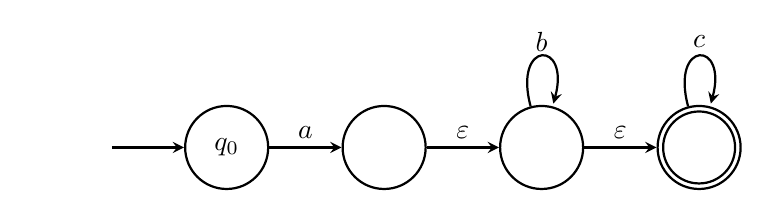
\begin{tikzpicture}
    \begin{scope}[auto, every node/.style={thick, draw,circle,minimum size=3em,inner sep=1}]
                        \node [draw=none] (I) at (-2,0) {};
                        \node (q0) at (0,0) {\(q_0\)};
                        \node (a) at (2,0) {};
                        \node (b) at (4,0) {};
                        \node (c) at (6,0) {};
                        \draw[black, thick] (6,0) circle [radius=1.3em];
                \end{scope}

                \begin{scope}[auto, every node/.style={minimum size=1em,inner sep=1}, every path/.style={thick, ->, >=stealth}]
                        \path (I) edge (q0);
                        \path (q0) edge node {\(a\)} (a);
                        \path (a) edge node {\(\varepsilon\)} (b);
                        \path (b) edge [loop above] node {\(b\)} (b);
                        \path (b) edge node {\(\varepsilon\)} (c);
                        \path (c) edge [loop above] node {\(c\)} (c);
               \end{scope}
\end{tikzpicture}
\end{center}

\newpage

\section{}
$L_3 := \{a^ib^jc^k \,|\, i > j + k\}$ is a non-FSL CFL. The (N)PDA is given below.

\begin{center}
    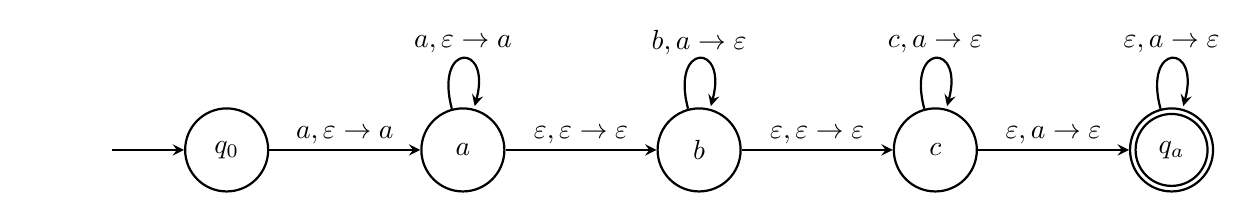
\begin{tikzpicture}
        \begin{scope}[auto, every node/.style={thick, draw, circle, minimum size=3em, inner sep = 1}]
            \node [draw=none] (I) at (-2,0) {};
            \node (q0) at (0,0) {\(q_0\)};
            \node (a) at (3,0) {\(a\)};
            \node (b) at (6,0) {\(b\)};
            \node (c) at (9,0) {\(c\)};
            \node (ac) at (12,0) {\(q_a\)};
            \draw[black, thick] (12,0) circle [radius=1.3em];
        \end{scope}
        \begin{scope}[auto, every node/.style={minimum size=1em,inner sep=1}, every path/.style={thick, ->, >=stealth}]
            \path (I) edge (q0);
            \path (q0) edge node {\(a, \varepsilon \rightarrow a\)} (a);
            \path (a) edge [loop above] node {\(a, \varepsilon \rightarrow a\)} (a);
            \path (a) edge node {\(\varepsilon, \varepsilon \rightarrow \varepsilon\)} (b);
            \path (b) edge [loop above] node {\(b, a \rightarrow \varepsilon\)} (b);
            \path (b) edge node {\(\varepsilon, \varepsilon \rightarrow \varepsilon\)} (c);
            \path (c) edge [loop above] node {\(c, a \rightarrow \varepsilon\)} (c);
            \path (c) edge node {\(\varepsilon, a \rightarrow \varepsilon\)} (ac);
            \path (ac) edge [loop above] node {\(\varepsilon, a \rightarrow \varepsilon\)} (ac);
        \end{scope}
    \end{tikzpicture}
\end{center}

\noindent
The PDA above ensures that at least one $a$ is in the input string (since even if $j = k = 0$, $i \geq 1$ since $0 \not> 0$). After that, we push an $a$ onto the stack for each input symbol $a$. We allow epsilon-transitions for the $b$ and $c$ states since it is possible for $j = k = 0$. For each $b$ or $c$ encountered, we pop an $a$ from the stack. If at any point, we read a $b$ or $c$ and there are no more $a$'s on the stack, then we block and fail to accept. Additionally, to get to the accepting state $q_a$, we require there be at least one $a$ on the stack remaining, since $i \neq j + k$. We loop forever and accept as long as there are remaining $a$'s, since we can have unbounded occurrences of $a$.

\newpage

\section{}
$L_4$ is not a CFL. To prove by contradiction, assume that $L_4$ is a CFL. Per the pumping lemma for CFLs, there is some pumping length $p$ such that for any string $s$ such that $|s| \geq p$, $s := uvxyz$. $\forall{(i \geq 0)} (uv^ixy^iz \in L_4)$, $|vy| > 0$, and $|vxy| \leq p$.

\noindent
Consider the string $s_p = a^{2p}b^pc^{2p}$. $|s| = 5p > p$ and $s \in L_4$ since the number of $a$'s and the number of $c$'s are equal and twice the number of $b$'s. Since $|vxy| \leq p$ and $|vy| > 0$, we know that there are two broad possibilities to consider: either $vy$ consists of the same symbol or it does not. If $vy$ consists of the same symbol, then when $i = 0$, the resulting string $s' \not\in L_4$. To show this, consider all possible cases from $\Sigma$:

\begin{itemize}
    \item $a$ - When $i = 0$, $s' = uxz = a^{2p - |vy|}b^pc^{2p}$ i.e. $\#(a,s') \neq \#(c, s')$.
    \item $b$ - When $i = 0$, $s' = uxz = a^{2p}b^{p - |vy|}c^{2p}$ i.e. $\#(a, s') \neq 2 \cdot \#(b,s')$
    \item $c$ - When $i = 0$, $s' = uxz = a^{2p}b^pc^{2p - |vy|}$ i.e. $\#(c,s') \neq \#(a, s')$.
\end{itemize}

\noindent
If either $v$ or $y$ consists of different symbols, notice it is not possible for $vy$ to consist of more than two symbols since $|vy| \leq p$ and the substrings are all of at least length $p$. Therefore, there are three cases once again for the value of $vy$:

\begin{itemize}
    \item No $c$'s - Thus, $vy$ consists of $a$'s and $b$'s. Because of this, consider when $i = 0$, then $s' = uxz$ and $\#(a,s') \neq \#(c,s')$ because $vy$ consists of some non-zero number of $a$'s and cannot be long enough to consist of any amount of $c$'s.
    \item No $a$'s - Thus, $vy$ consists of $b$'s and $c$'s. Similar logic as above follows i.e. $\#(c,s') \neq \#(a,s')$ because there is some non-zero amount of $c$'s removed when $i = 0$.
    \item No $b$'s - This option is not possible since $|vy| \leq p$ and since there are $p$ occurrences of $b \in s'$, it is not possible for both $a$ and $c$ to be in $vy$.
\end{itemize}

\noindent
Thus, as no possible partition of $s'$ holds for \textit{all} values of $i$, $s' \not\in L_4$ and thus $L_4$ cannot be a CFL since it does not obey the pumping lemma.

\end{document}
